\begin{frame}
  \frametitle{Results for the Previous Week}

  \begin{center}
    Here are the results for last week:

    \bigskip
    
    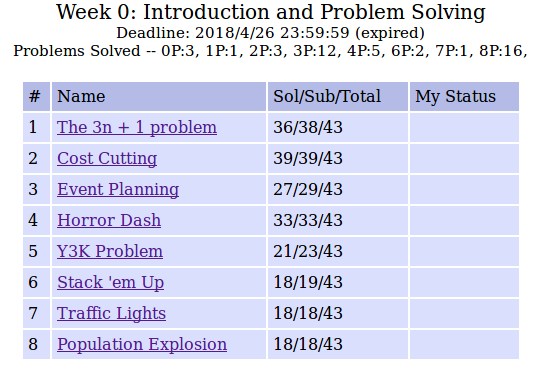
\includegraphics[width=0.8\textwidth]{img/resultW0}
    
    \bigskip

    Hope you enjoyed the warm up!
  \end{center}

\end{frame}

\begin{frame}[fragile]
  \frametitle{More about input...}

  Do not enter the input by hand! Create an input file, and run your
  program with the input file to save time and get more precise
  results.

  \bigskip

  \begin{block}{}
\begin{verbatim}
$ cat - > input.in
1 10
10 1
10 10 
$ g++ 100.cpp
$ ./a.out < input.in
1 10 20
10 1 20
10 10 7
\end{verbatim}
  \end{block}
  
\end{frame}

%\begin{frame}
%  \frametitle{Comments about the problems}
%\end{frame}
